\documentclass[letterpaper, 12pt]{article}

 
\usepackage[utf8]{inputenc}
\usepackage[T1]{fontenc} 
\usepackage[french]{babel}
\usepackage{amsmath}
\usepackage{textcomp}
\usepackage{tocloft}

\usepackage[letterpaper, left=2.5cm, right=2.5cm, top=2.5cm, bottom=2.5cm]{geometry}
\usepackage{graphicx}
\usepackage{float} 
\usepackage{setspace} 
\usepackage{fancyhdr}      
\usepackage{cite}

\usepackage[pdftex, colorlinks=true, linkcolor=black, citecolor=blue]{hyperref}

\title{Proposé de recherche}
\author{Thomas Dändliker}
\date{\today}

\pagestyle{fancy}
\fancyhead[L]{Proposé de recherche}
\fancyhead[R]{MET-7900}

%%%%%%%%%%%% Fin du préambule %%%%%%%%%%%

\begin{document}

\begin{titlepage}
	\newcommand{\HRule}{\rule{\linewidth}{0.2mm}}     
	
	\begin{figure}[t]
		\begin{minipage}{0.5\textwidth}\large
			\begin{flushleft}
				
\includegraphics[width=5cm]{ULAVAL}
			\end{flushleft}
		\end{minipage}
		\begin{minipage}{0.5\textwidth}\large
			\begin{flushright}
				
\includegraphics[width=6cm]{CRMR}
				
			\end{flushright}
		\end{minipage}
	\end{figure}
	\textsc{ \\[1cm]}
	
	% Titre
	\begin{center}
		\HRule 
		\\[0.5cm]
		{\Large    \textbf{Optimisation de la densité de reboisement en fonction des grades de qualité des bois sciés}}
		\HRule
		\\[0.5cm]
		{\large Proposé de recherche \\
		}
		
	\end{center}
	
	\vfill 
	\begin{center}
		
		\textsc{\large      
			Université Laval\\
			Faculté de foresterie, de géographie et de géomatique\\[3cm]}
	\end{center}

	
	\begin{minipage}{0.5\textwidth}
		\begin{flushleft} \large
			\emph{Auteur:}\\
			Thomas Dandliker 
		\end{flushleft}
	\end{minipage}
	~
	\begin{minipage}{0.5\textwidth}
		\begin{flushright}\large
			\emph{Superviseurs:} \\
			Alexis Achim \\
			Charles Ward \\
		\end{flushright}
	\end{minipage}
	
\end{titlepage}


\renewcommand{\contentsname}{\hfill\bfseries\LARGE Table des matières\hfill} 
\renewcommand{\listfigurename}{\hfill\bfseries\LARGE Table des figures\hfill} 

%%%%%%%%% Table des matières %%%%%%%%%%%

\newpage
\doublespacing
\setcounter{tocdepth}{3}
\tableofcontents
\addtocontents{toc}{\vspace{2cm}}

%%%%%%%%% Table des figures %%%%%%%%%%

\newpage
\doublespacing
\listoffigures

\newpage
\section{Introduction}
\begin{onehalfspace}

Les forêts issues de plantation comptent pour 4\% des forêts mondiales, mais fournissent, à elles seules, 50\% de la production de bois \cite{Miller2009}. Pour la période de 2001 à 2012, avec environ 120 millions de plants plantés annuellement, les résineux représentent presque la totalité des plantations au Québec, soit 98\% \cite{Richard2015}. Depuis 2001, 94\% des plantations sont réalisées avec trois essences: l'épinette noire (56\%), le pin gris (21\%) et l'épinette blanche (17\%) comme l'illustre la figure 1. 

\vspace{12pt}

\begin{figure}[h]
	\centering
	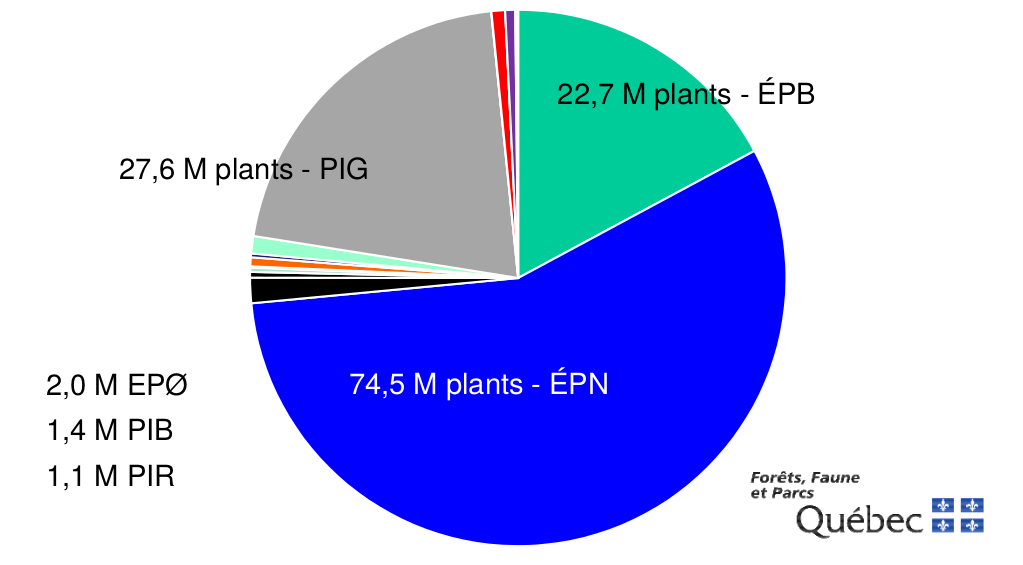
\includegraphics[width=12cm]{Essencesplantees}
	\caption{Essences plantées entre 2001 et 2012 au Québec}
\end{figure}


Ces trois essences font partie du groupe dits SEPM (Sapin, Épinettes, Pins, Mélèzes), qui constitue la  majeure  partie  des  volumes  de  bois  récoltés et transformés au Québec. Ce groupe est à la base de l’approvisionnement des usines produisant du sciage\cite{Gouv2017}. Dans un marché globalisé, cela implique d'optimiser les procédés qui englobent toutes la chaîne de valeur du bois, y compris les scénarios sylvicoles \cite{Gaudreault2010}. 

\vspace{12pt}

Dans ce cadre de rationnalisation, la densité de plantation est un outil ayant une influence importante en sylviculture, puisqu'elle détermine la croissance et les caractéristiques du peuplement \cite{Thiffault2003}. De manière générale, la hauteur dominante, quant à elle, n'est pas influencée par l'espacement entre les tiges \cite{Gizachew2012}. En revanche, lorsque le nombre de tiges par hectare augmente, on a pu observer des augmentations du volume total et de la surface terrière, et, dans le même temps, une diminution du diamètre quadratique moyen. De plus, la mortalité y est aussi plus forte, due à une compétition intraspécifique plus élevée \cite{Groot2016, Will2010}. À l'inverse, à plus faible densité de plantation, on constate un taux de survie plus élevé, ainsi qu'une plus forte croissance en diamètre et en volume par tige \cite{Akers2013}. On y observe également une augmentation du défilement. Ce dernier aspect a une incidence directe sur le volume marchand des tiges. En effet, pour un même diamètre donné, un défilement plus élevé diminue le volume marchand à l'échelle de l'arbre\cite{Pregent1998}. Ainsi, deux facteurs entrent en compte lors de la première transformation d'un arbre: le diamètre et la hauteur totale. Ces deux caractéristiques influent sur la composition du panier de produits sciés \cite{Auty2014}, comme par exemple la proportion de sciage. 

\vspace{12pt}

Aussi, l'accroissement plus élevé que l'on constate en plantation modifie les caractéristiques du bois et, de ce fait, a un effet déterminant quant à la valeur et à l'utilisation finale du produit \cite{Zhang2002}. Une manière d'attribuer une valeur pour les résineux consiste à effectuer un classement visuel des bois sciés comme le fait la norme "National Lumber Grades Authority (NLGA)". Les nœuds (branches), notamment leurs tailles et leurs nombres, sont des caractéristiques importantes à prendre en considération lors du classement des bois sciés \cite{Lemieux2000}. 

\vspace{12pt}

Dans la littérature, un certain nombre d'études soulignent le fait que le DHP de l'arbre a davantage d'effet sur les caractéristiques des branches, que l'espacement initial. Ainsi, les attributs des nœuds peuvent être prédits pour le pin gris et l’épinette noire à partir de données externes de branches, notamment le diamètre des branches \cite{Duchateau2013}. De plus, pour un site donné, les propriétés des noeuds d'épinette noire (\textit{Picea mariana} (Mill.)) sont relativement peu sensibles à l'espacement des arbres, car elles sont largement expliquées par la taille du fût et celle du houppier \cite{Benjamin2009, Zhang2005}. Cela est également observé sur l'épinette de Norvège en Scandinavie \cite{Johansson1992, Makinen1999, Pfister2007}. Enfin, le diamètre de la plus grande branche est positivement corrélé au DHP de l'arbre, quel que soit l'espacement entre les arbres \cite{Hebert2016, Tong2005}. 

\vspace{12pt}

Il est également reconnu que le DHP d'un arbre est, à son tour, étroitement lié à la densité de plantation \cite{Pregent1998}. Plusieurs études vont dans ce sens. Pour le pin gris (\textit{Pinus banksiana} Lamb.), l'espacement des plantations a un effet significatif sur le plus grand diamètre de la branche pour les pins gris dominants \cite{Hebert2016}. Enfin, pour l'épinette blanche (\textit{Picea glauca}), un espacement plus large entre les arbres a tendance à augmenter la largeur des nœuds \cite{Tong2013}. Aux vues de ces connaissances, le sylviculteur a une réelle emprise sur la qualité du bois dès sa première décision, qui est celle de choisir la densité de plantation.

\vspace{12pt}

Les études menées préalablement sur les branches sont, pour l'instant, toutes limitées à un site en particulier avec des conditions de croissance bien définies (indice de qualité de station, précipitation, température...). La présente étude s’appuie sur un réseau de placettes permanentes à l’échelle de la province du Québec, ce qui permettra de couvrir de nombreux sites ayant des conditions de croissance différentes. En outre, les études évaluant la proportion de sciage proviennent de jeunes peuplements résineux qui ne sont pas encore arrivés à maturité; donc n’ayant pas suivi un scénario sylvicole complet, avec ou sans éclaircies. 

\vspace{12pt}

De facon générale, l'association de la taille des nœuds et du défilement peut influer sur la qualité du bois. Toutefois, cette conclusion est appuyée sur des données fragmentaires, notamment sur des arbres d'une trentaine d'années dans les plantations boréales. Le présent projet vise à établir un lien entre la futur qualité du bois scié et la croissance des arbres à différents espacements pour trois espèces commerciales du Canada, soient l'épinette noire, l'épinette blanche et le pin gris. L'objectif de l'étude est d'évaluer l'effet de différents espacements sur les propriétés du bois d'arbres arrivés à maturité. Plus particulièrement, nous avons cherché à déterminer si une réponse positive du DHP à un espacement plus grand affecterait le classement du bois et la proportion de sciage.

\vspace{12pt}

Nous avons émis l'hypothèse qu'une densité de reboisement plus faible augmenterait le diamètre à l'échelle de l'arbre, ce qui, à son tour, impacterait le rendement de sciage en augmentant la proportion de sciage de la tige. La deuxième hypothèse suppose que la mortalité observée à plus forte densité soit un facteur de déclassement de la qualité du bois en augmentant la grosseur des noeuds. 

\section{Matériels et méthodes}

\subsection{Aire d'étude}

L'expérience a lieu à l'échelle de la province du Québec, en se basant sur le réseau des placettes permanentes de la Direction de la Recherche Forestière (DRF). Les essences étudiées sont l'épinette noire (\textit{Picea mariana} (Mill.)), l'épinette blanche (\textit{Picea glauca}) et le pin gris (\textit{Pinus banksiana} Lamb.). Les mesures sont prises à l'été et automne 2018 ainsi qu'au printemps et été 2019 dans une centaine de plantations monospécifiques âgées de 30 ans environ. Aucune éclaircies précommerciales n'a eu lieu dans ces plantations. 

La placette permanente est une unité d'échantillonnage circulaire d'une superficie de 400 m$^{2}$ \cite{MFFP2016}. Dans le cadre de ce projet, les données suivantes ont été relevées sur un nombre déterminé d'arbres: essence de l'arbre, le diamètre à hauteur de poitrine (DHP) et les caractéristiques de la plus grosse branche sur les 5 premiers mètres de la tige. 

\subsection{Mesures de branches}

La classification des branches se fait d’abord sur les arbres études compris dans les étages dominants et codominants (8 à 10 arbres par parcelle) et, en second, sur les arbres listés dans le formulaire électronique de DendroDIF. En prévision que certains arbres aient par exemple des défauts non présents lors du dernier mesurage, la liste identifie tous les arbres respectant les quatre critères de sélection. La liste sert à compléter la sélection des arbres jusqu’à une concurrence de 20 arbres et elle n’est pas triée en ordre prioritaire de sélection. Les arbres sont sélectionnés prioritairement sur la ligne à proximité du centre de la parcelle (ligne en rouge et pleine sur la Figure 1), suivi sur la ligne le plus vers le nord magnétique, suivi sur les lignes adjacentes jusqu’à atteindre la ligne centrale de la parcelle  (lignes en bleu sur la Figure 1) et, si nécessaire, sur les autres lignes adjacentes à la ligne du centre et en priorisant toujours celles orientées vers le nord magnétique (lignes en jaune sur la Figure 1).

\vspace{12pt}

\begin{figure}
	\centering
	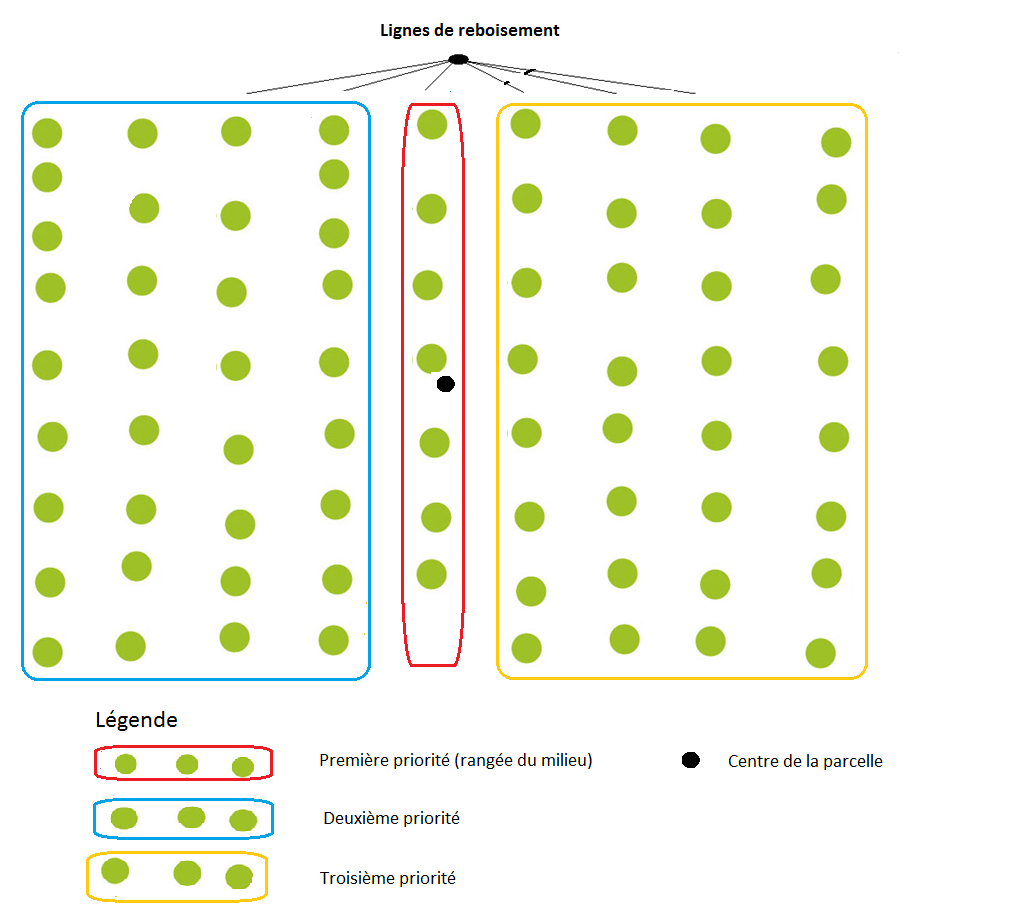
\includegraphics[width=10cm]{Figure1}
	\caption{Priorité de sélection des arbres pour la classification des branches}
\end{figure}

La circonférence de la bille de pied de 4,9 m (16 pieds) est divisée en quatre faces égales (Figure 2). Les faces A et C sont alignées sur la ligne de plantation et les faces B et D sont perpendiculaires à la ligne de plantation. La face A est celle orientée le plus vers le nord magnétique et elle est identifiée par un trait de peinture vertical de 10 cm, à la base du tronc, à l’aide de peinture.

\vspace{12pt}

\begin{figure}[H]
	\centering
	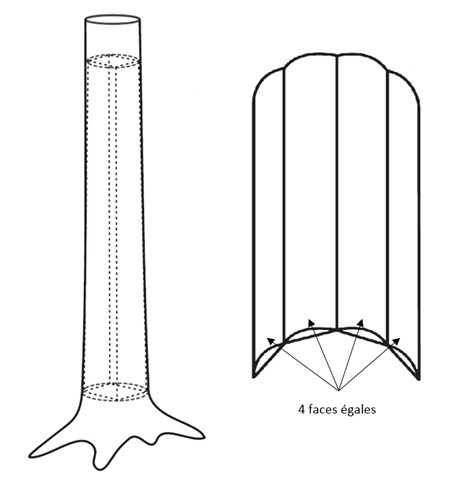
\includegraphics[width=6cm]{Figure2}
	\caption{Division de la circonférence de la bille de pied en quatre faces égales}...
\end{figure}

\vspace{12pt}

Le diamètre de la plus grande branche est mesuré sur chacune des faces, selon les six classes suivantes :

\begin{figure}[H]
	\centering
	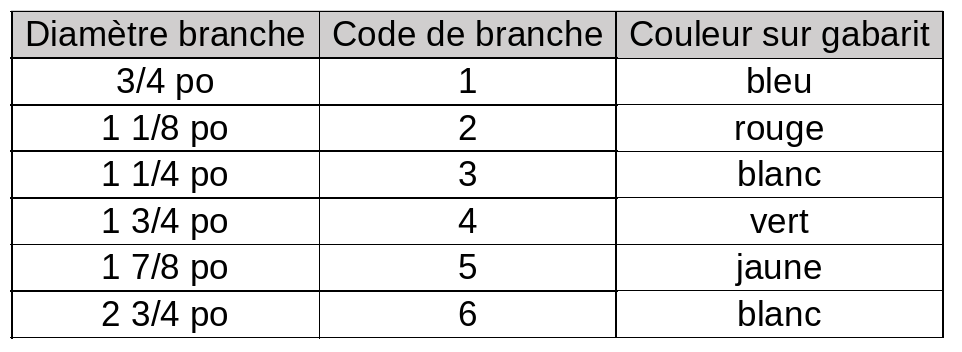
\includegraphics[width=10cm]{Code}
\end{figure}

\vspace{12pt}

La plus grosse branche est sélectionnée jusqu’à une hauteur de 5,23 m (17 pieds), à partir du sol, et elle est classifiée à l’aide du gabarit métallique. À cet effet, des perches télescopiques et des gabarits métalliques, identifiant les six classes de diamètres de branches, sont fournis à l’entrepreneur.

\vspace{12pt}

La mesure des branches se décline comme suit:

\begin{enumerate}
	
\item Déployer la perche téléscopique pour atteindre une longueur de 3,93 m. Cette longueur correspond à la longueur totale de la perche sans le gabarit. Ainsi elle débute au niveau du trait rouge présent sur le gabarit métallique (Figure 4) jusqu'à l'autre extrémité de la perche téléscopique.

\item Se placer devant la face à mesurer avec la perche téléscopique munie du gabarit métallique.

\item Positionner la base de la perche à  1,3 m du sol : prendre la perche téléscopique par la base, et la soulever jusqu'au niveau du DHP, identifié par un trait de peinture sur l'arbre (Figure 5). Cette position permet de délimiter la hauteur totale de 5,23 m, hauteur qui sert à étudier les branches.

\item Chercher la branche la plus grosse sur la face étudiée et la mesurer à l’aide du gabarit métallique (Figure 4). Inscrire dans le formulaire Dendrodif le «code diamètre branche» selon le tableau ci-dessus (Tableau 1), correspondant à la plus grosse branche. Pour chacune des branches, identifier et inscrire dans le formulaire Dendrodif, son «état branche» : vivante = \textbf{V}, ou morte = \textbf{M}.  De plus, inscrire dans le formulaire Dendrodif, son «angle insertion branche» : 45° et moins = \textbf{- 45}, ou 45° et plus = \textbf{+ 45}.

\end{enumerate}

\vspace{12pt}
 
Voir exemple ci-dessous de prise de mesures dans le formulaire Dendrodif :

\begin{figure}[H]
	\centering
	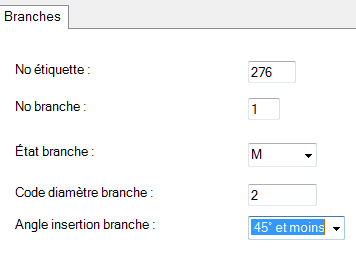
\includegraphics[width=5cm]{Figure3}
	\caption{Interface DendroDif}
\end{figure}

\begin{figure}[H]
	\centering
	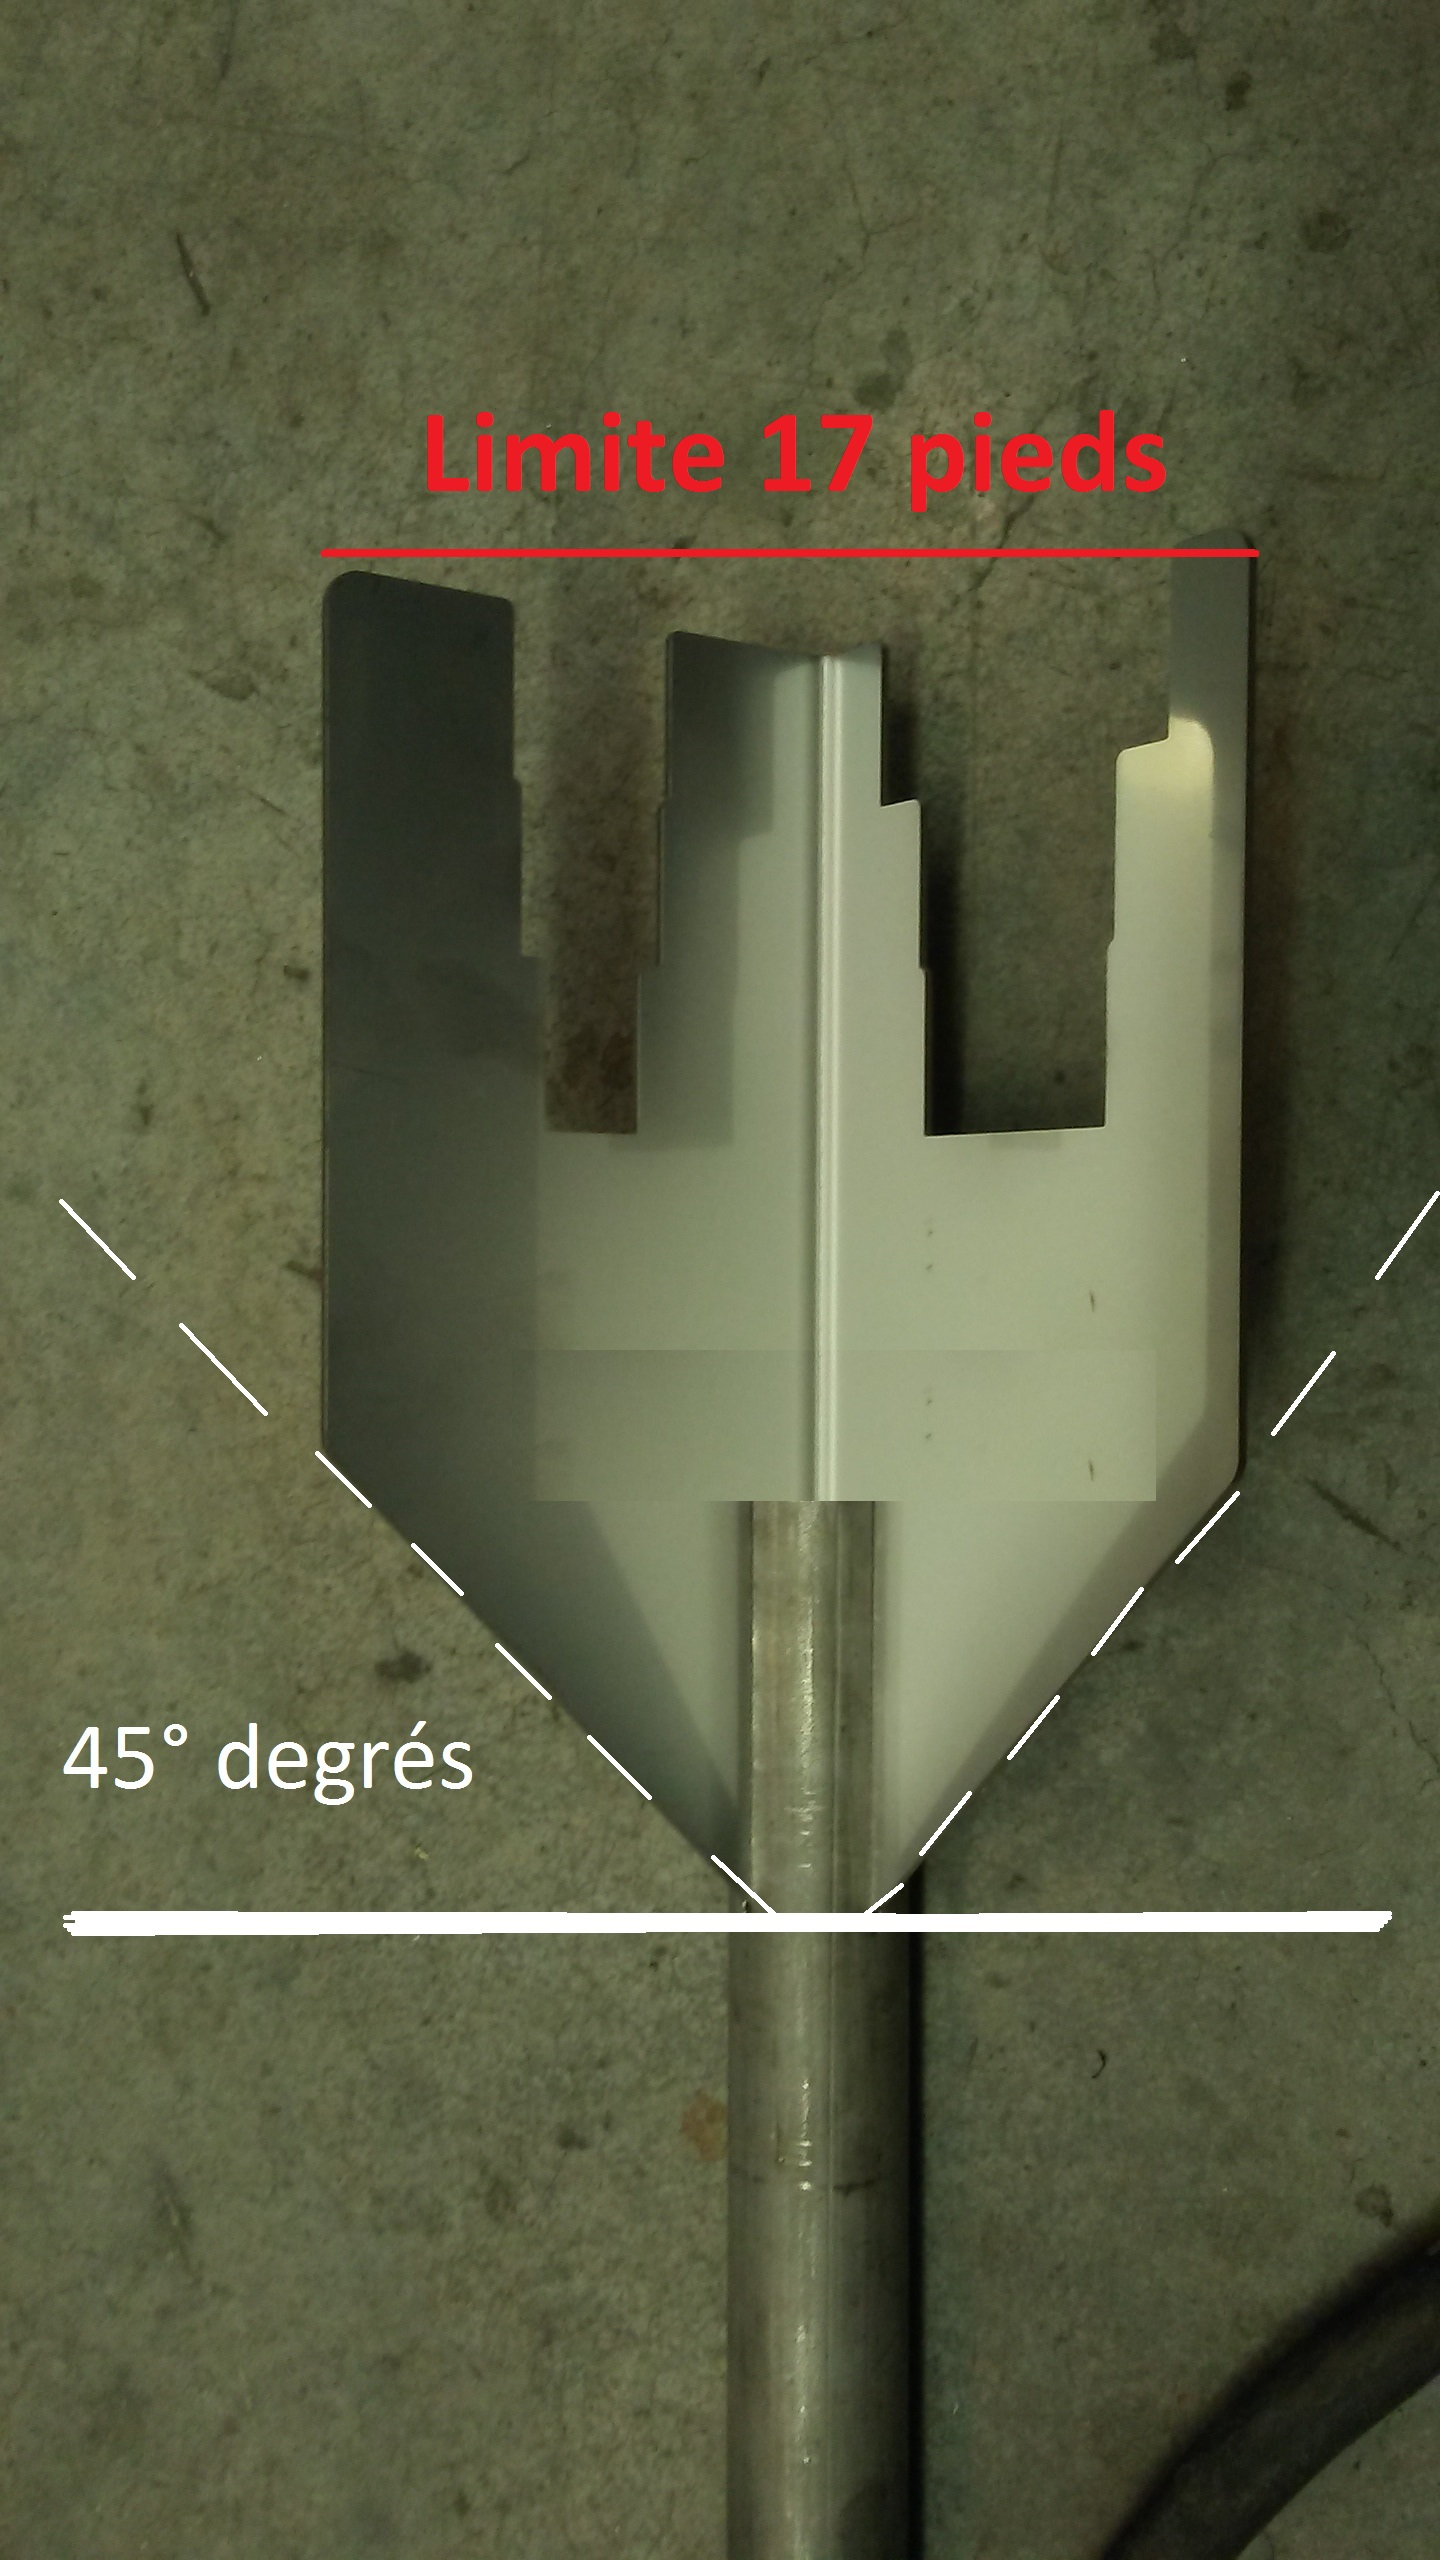
\includegraphics[width=5cm]{Figure4}
	\caption{Gabarit métallique}
\end{figure}

\begin{figure}[H]
	\centering
	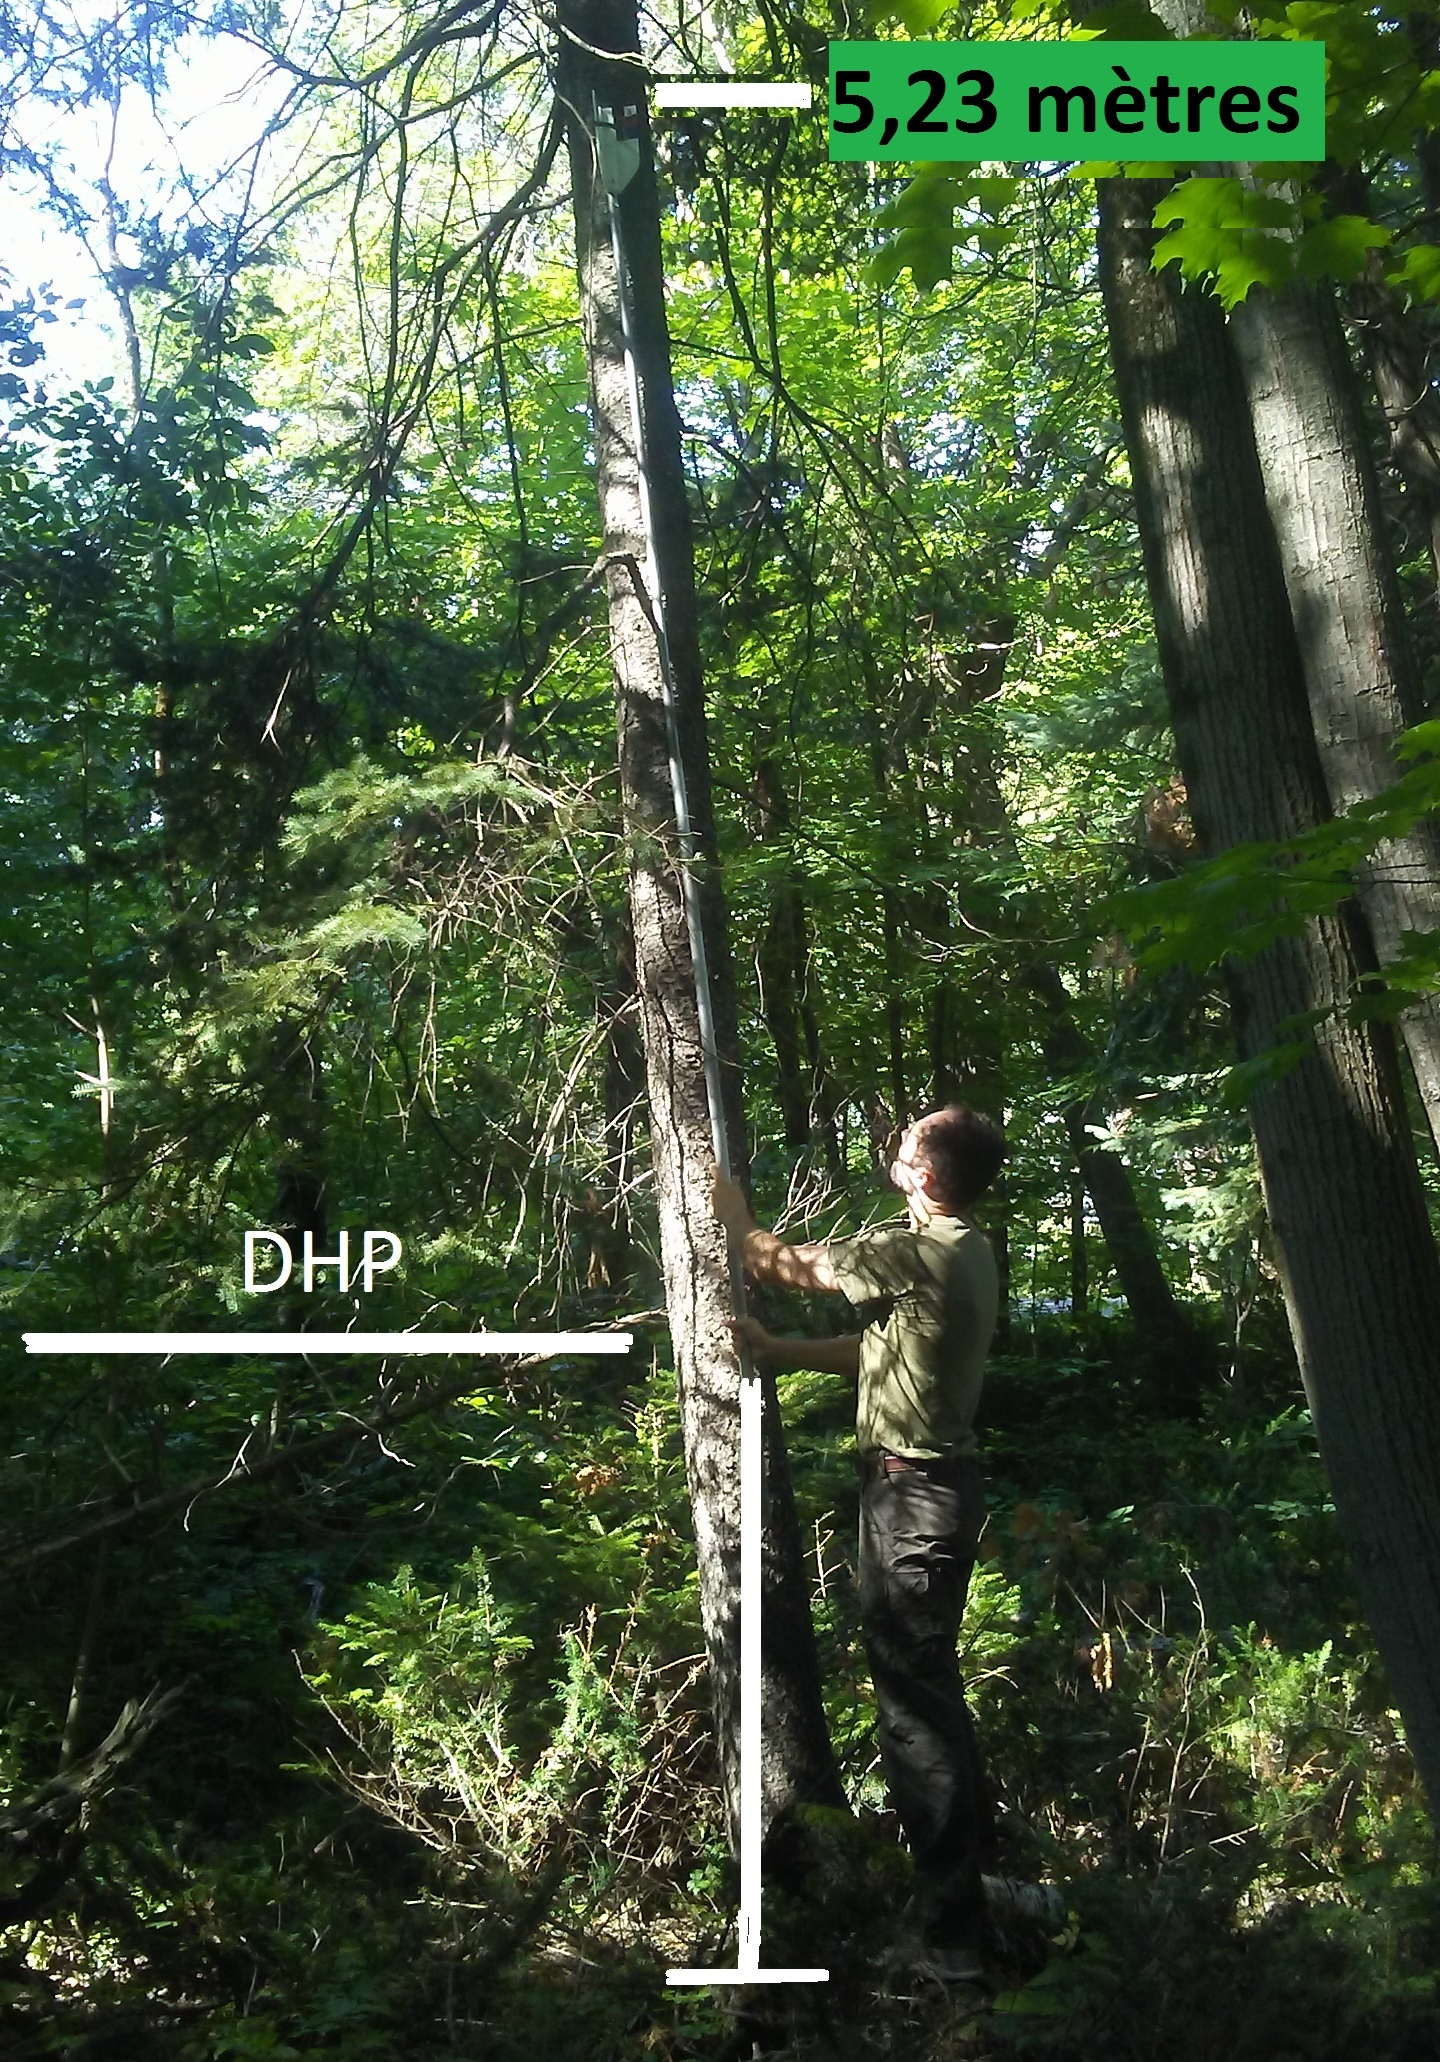
\includegraphics[width=5cm]{Figure5}
	\caption{Détermination de la hauteur de 5,23 m}
\end{figure}

\subsubsection{Analyse statistique}

Plusieurs données seront récoltées sur les arbres dans toutes les placettes permanentes. Pour l'analyse de ces données, les variables dépendantes seront les suivantes: le numéro d'encoche (grosseur de la branche), l'inclinaison de la branche, et l'état de la branche. Quant aux variables explicatives, il y aura : l'essence, la densité de plantation (plant/ha), l'IQS et l'exposition. Concernant les paramètres environnementaux, nous utiliserons principalement l'exposition, car elle peut favoriser la croissance du houppier sur la face la plus ensoleillée. 

\subsection{Modélisation du défilement}

À l’aide d’un simulateur d’éclaircies créé par la Direction de la Recherche Forestière (Guy Prégent), il sera possible de déterminer le DHP quadratique et la hauteur dominante des tiges à maturité en fonction: de l’essence, de l’IQS, de la densité de reboisement et du scénario sylvicole (0, 1 ou 2 éclaircies). 

\subsection{Modélisation du panier de produit}

Dans un contexte de marché de plus en plus compétitif, et où les coûts d'extraction pour la ressource et la fabrication des produits du bois augmentent, il devient primordial de maximiser la création de valeur lors de la première tranformation \cite{Briggs2010, Walker2013}. Depuis plusieurs décénnies, des simulateurs informatiques de sciages sont utilisés dans le secteur des transformations primaire et secondaire comme stratégie pour optimiser la valeur des produits \cite{FPInnovations2014}. Plusieurs études ont intégré avec succès les variabilités de la taille des arbres (tels que le diamètre de la tige, la hauteur totale de l’arbre ou la conicité de la tige) dans des modèles permettant de prédire le volume ou la valeur lors de la transformation \cite{Barrette2012,Liu2007}. Parmi les simulateurs, FPInnovations a développé Optitek, un programme qui utilise les données acquises à partir de scanners laser pour donner une représentation tridimensionnelle de la forme réelle de la tige \cite{FPInnovations2014}. Des améliorations ont été apportées afin de tenir compte des caractéristiques réelles des arbres, par le biais du modèle statistique STATSAW, et ainsi prédire la composition du panier de produits sciés \cite{Auty2014}. Ce modèle est paramétré pour l'épinette noire. À défaut d'avoir d'autres modèles, nous utiliserons STATSAW aussi pour l'épinette blanche et le pin gris.

\section{Résultats escomptés}

On s’attend à une relation entre la densité de plantation et les propriétés du bois (proportion de sciage, grosseur des branches). Le défilement est bien documenté sur les trois essences, ce qui permettra de bien alimenter le simulateur Optitek en données pour prévoir une valeur par arbre. Les ajustements avec le modèle STATSAW étant initialement paramétrés pour l'épinette noire, il y aura nécessairement une incertitude pour l'épinette blanche et le pin gris quant à la projection du panier de produits. Toutefois, on suppose une augmentation de la proportion de sciage pour toutes les essences au fur et à mesure que la densité diminue. 

\vspace{12pt}
Pour le diamètre de la plus grosse branche, on s'attend à observer une augmentation de la grosseur des branches à de plus fortes densités. En effet, la hausse de la mortalité interspécifique devrait libérer de l'espace aux arbres résiduels et favoriser leurs développement de houppier et donc des branches. 





\section{Conclusion}

À la lumière des résultats obtenus, des recommandations pourront être formulées auprès des praticiens en régions pour les sensibiliser aux effets de la densité de reboisement sur les caractéristiques du bois. En  termes  économiques,  si  les caractéristiques du bois ne se dégradent pas trop rapidement au fur et à mesure qu'on diminue la densité de plantation,  il peut être envisageable d'abaisser le nombre de tiges à l'hectare et donc de réduire les  coûts  de  plantation. Une autre retombée espérée est de pouvoir créer, à long terme, des bois issus de plantations ayant le meilleur panier de produits possible. 

\end{onehalfspace}

\section{Échéancier}

\begin{figure}[H]
	\centering
	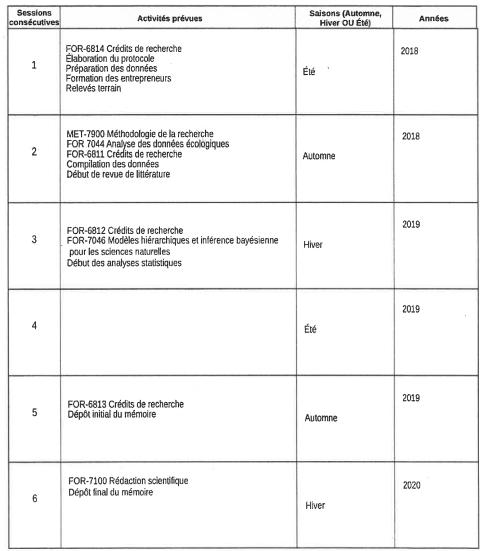
\includegraphics[width=15cm]{Calendrier}
	\caption{Calendrier des activités}
\end{figure}


\newpage

\nocite{*}
\bibliographystyle{unsrt}
\bibliography{biblio}

\end{document}